\chapter{Описание программы}

В данном разделе описывается функциональные возможности утилиты WEPfrag.

\section{Общие сведения}

Утилита WEPfragm, представленная в приложении~\ref{app:listing_fragmentation} и
приложении~\ref{app:listing_generate_arp_packet}, была разработана в
исследовательских академических целях, для практической проверки
работоспособности теоретических методов, описанных в разделе 3. Программа
реализует фрагментационную атаку на протокол WEP.

Программа ориентирована на ОС Linux, так как использует драйвера беспроводного
оборудования. 

Программа реализована на языке программирования С. Данная реализация может в
дальнейшем развиваться и агрегировать в себе другие атаки на беспроводные сети.

\section{Функциональное назначение}

Данная программа рассчитана исключительно на реализацию фрагментационной атаки
на протокол WEP.

\section{Описание логической структуры}

Основными функциями программы являются:

\begin{itemize}
    \item{Ожидание ARP-пакета и вычисление PRGA (do\_attack\_fragment, см.
    приложение~\ref{app:listing_fragmentation});}
    \item{Формирование ARP-запроса (arp\_forge, см. 
    приложение~\ref{app:listing_generate_arp_packet});}
    \item{Создание правильного зашифрованного WEP-пакета (create\_wep\_packet, см. 
    приложение~\ref{app:listing_generate_arp_packet}).}
\end{itemize}

На рисунке~\ref{fig:fragment_program_algo} продемонстрирован алгоритм работы
программы. При прослушивании среды обнаруживается WiFi-пакет, по длине пакета
определяется является ли он ARP-пакетом. Если является, то выделяем из него PRGA
и передаём PRGA в функцию генерации ARP-запроса. Сгенерированный пакет шифруем
на полученном PRGA и сохраняем в файл для дальнейшей отправки в сеть.

\begin{figure}
    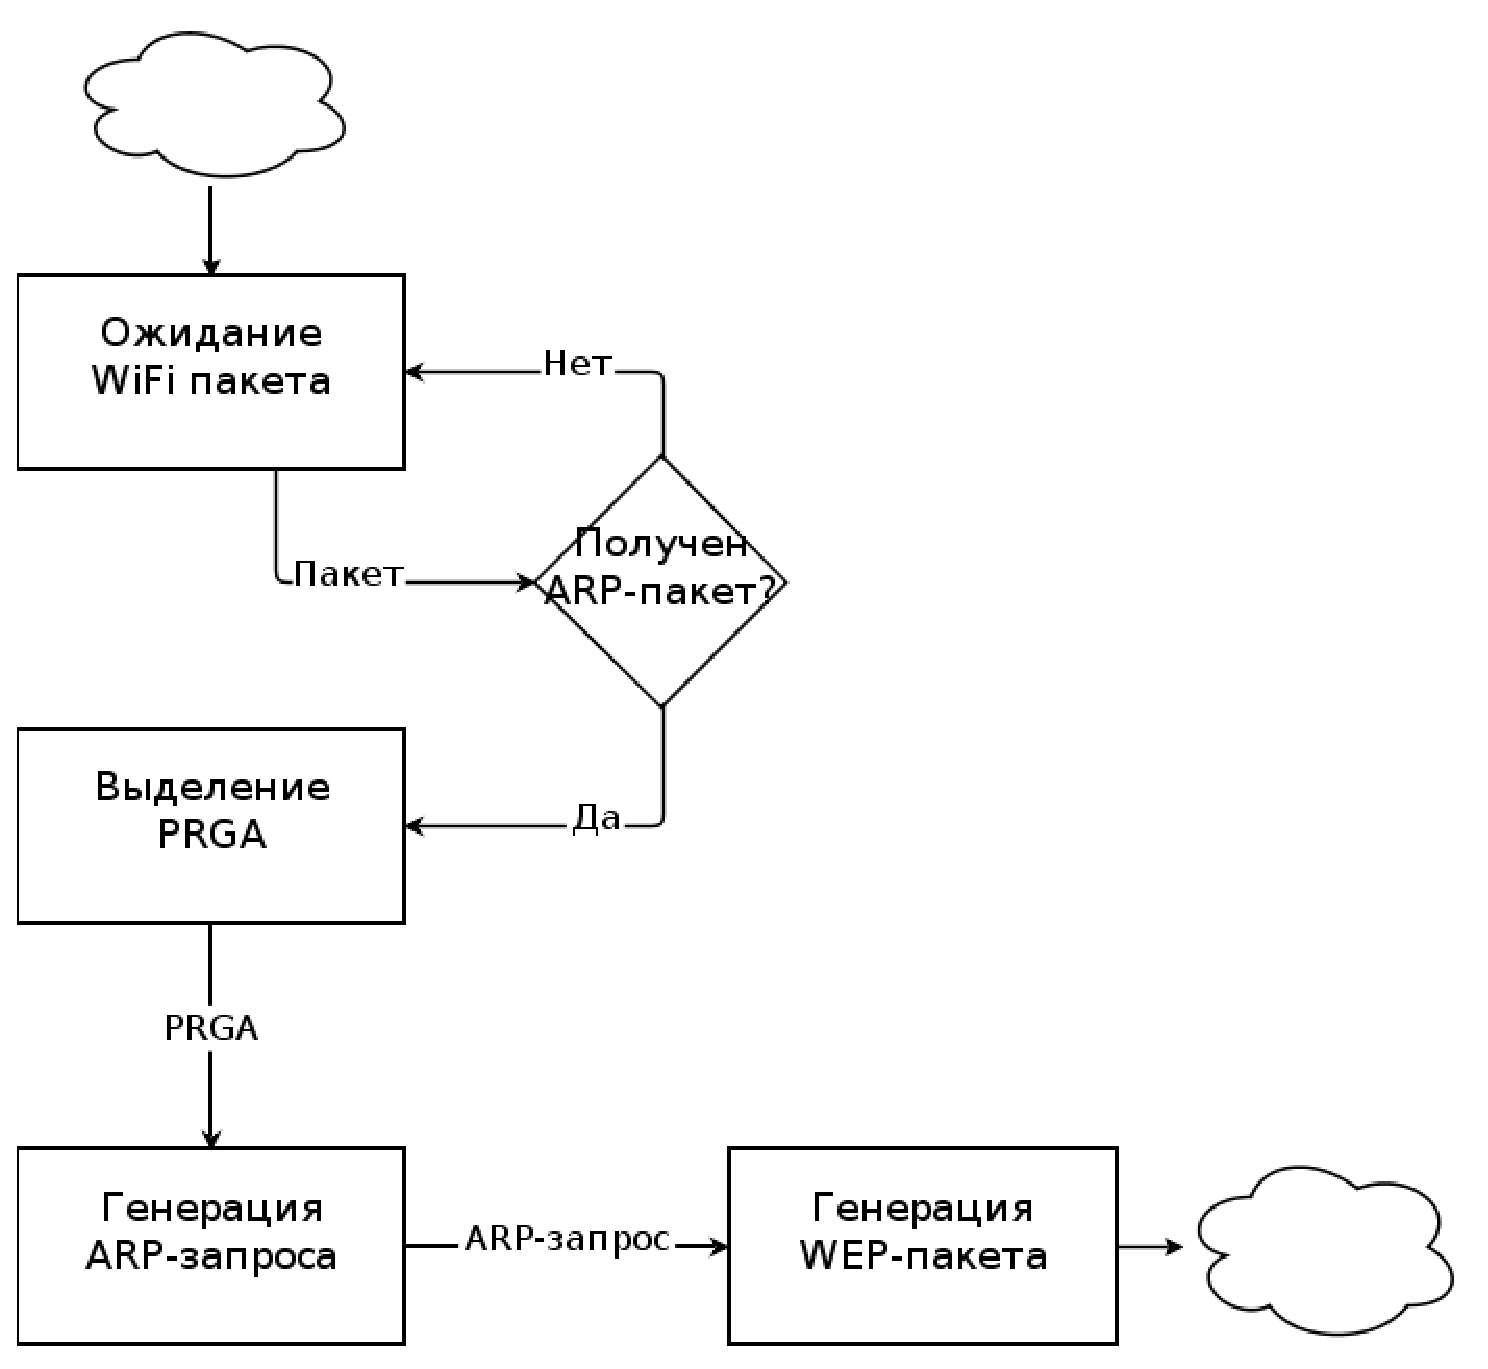
\includegraphics[width=1\textwidth]{graphics/fragment_program_algo.eps}
    \caption{Алгоритм работы программы}
    \label{fig:fragment_program_algo}
\end{figure}

Для запуска ожидания ARP-пакета и выделения PRGA используется функция:
int do\_attack\_fragment(uchar* prga).

Для генерации ARP-запроса используется:
int forge\_arp(uchar* prga).

Для создания шифрованного WEP-пакета используется:
int create\_wep\_packet(unsigned char* packet, int *length, uchar* prga).

\section{Используемые технические средства}

Для работы программы необходим ПК с установленной сетевой WiFi-картой, драйвера
которой поддерживают переход в режим мониторинга.

\section{Вызов и загрузка}

Утилита не принимает на вход никаких параметров, все необходимые парамеры были
константно заданы в утилите. В результате работы программы создаётся файл
arp\_replay, который является зашифрованным ARP-запросом.

\section{Входные и выходные данные}

Входными данными в программу являются перехваченные пакеты ARP.

Выходными данными является сформированный, зашифрованный ARP-запрос, который
можно отправлять в сеть для накопления большого количества векторов
инициализации.
